\subsection{Results on the DECam survey}
\label{sec:results_on_decam}

We next demostrate StarNet on a larger region of the sky.
The DECAPS survey imaged stars in our own Milky Way, and we chose
a $4000 \times 2000$ frame centered at coordinates $\text{RA} = 266.044^\circ$ and
$\text{DECL} = -28.88111^\circ$. See \ref{fig:decaps_ex} for an example image.

The DECAPS image is somewhat sparser than M2.
Thus, we set our Poisson mean parameter
smaller than on M2 (TODO give numbers), and
used a tile size of $10\times 10$ pixels with $30\times30$
padded tiles. We found that the same SGD converged after
100 epochs.
The fitting procudure took approximately 10 minutes; after the fit,
we produced
a color magnitude diagram for the full $4000 \times 1000$ frame,
consisting of $\sim 10,000$ stars, in $\sim 5$ seconds (Figure~\ref{fig:decaps_cmd}).
On the other hand, extrapolating the runtime of PCAT, running MCMC on this frame
would take on the order of days.


\begin{figure}[tb]
    \centering
    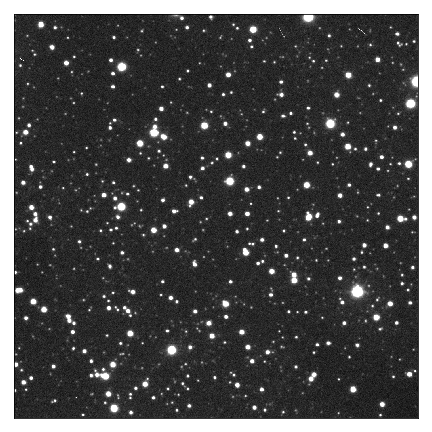
\includegraphics[width=0.8\textwidth]{./figures/decaps/example_subimage1000_decaps.png}
    \vspace{-0.4cm}
    \caption{A 1000 x 1000 pixel subregion of the DECAM survey. }
    \label{fig:decaps_ex}
\end{figure}

\begin{figure}[tb]
    \centering
    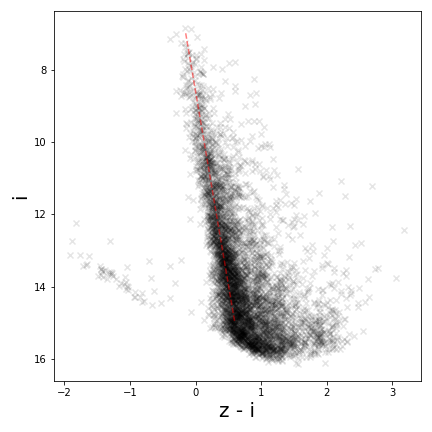
\includegraphics[width=0.4\textwidth]{./figures/decaps/decaps_cmd.png}
    \vspace{-0.4cm}
    \caption{Color magnitude diagram for the Decaps image. Red dashed line highlights
    the inferred blue main-sequence stars.
    }
    \label{fig:decaps_cmd}
\end{figure}
